\chapter{Introduction}
\label{ch:introduction}
\graphicspath{ {chapters/Introduction/} }

Streamlined manufacturing process always been an important factor for the success of a manufacturer in the market. 
Quality of the product, however, does not necessarily lead to high profit, which is essential for the company to grow. 
A product is profitable only if it can be produced with a lesser production cost than the market price. 
While the price is controlled by the market, the cost is easier to positively influence by improving the efficiency of the manufacturing system. 
Modern manufacturing is highly automated and consists of robotic cells which can produce parts even without an intervention of a human in some cases \cite{VirtualCommisioning}. \\

When developing a new product the engineers usually create a computer model of the product and based on that they can build prototypes. After the product is refined a different engineering team is tasked with designing an assembly line that could mass produce the parts and assemble them together. \\
 
Currently, assembly lines are designed in a specific type of CAD software, which allows the simulation of the full assembly sequence.
This way the engineers can validate the reachability and collision clearance of the prepared line, including human factors.
One example of such software is the Tecnomatix suite by SIEMENS. Tecnomatix Process Simulate (see Figure~\ref{fig:ProcessSimulate}) is an industry leading software for digital manufacturing, used by the likes of Volkswagen or Samsung \cite{TecnomatixCustomers}. \\ 

\begin{figure}[ht]
	\caption{Process Simulate}
	\centering
	  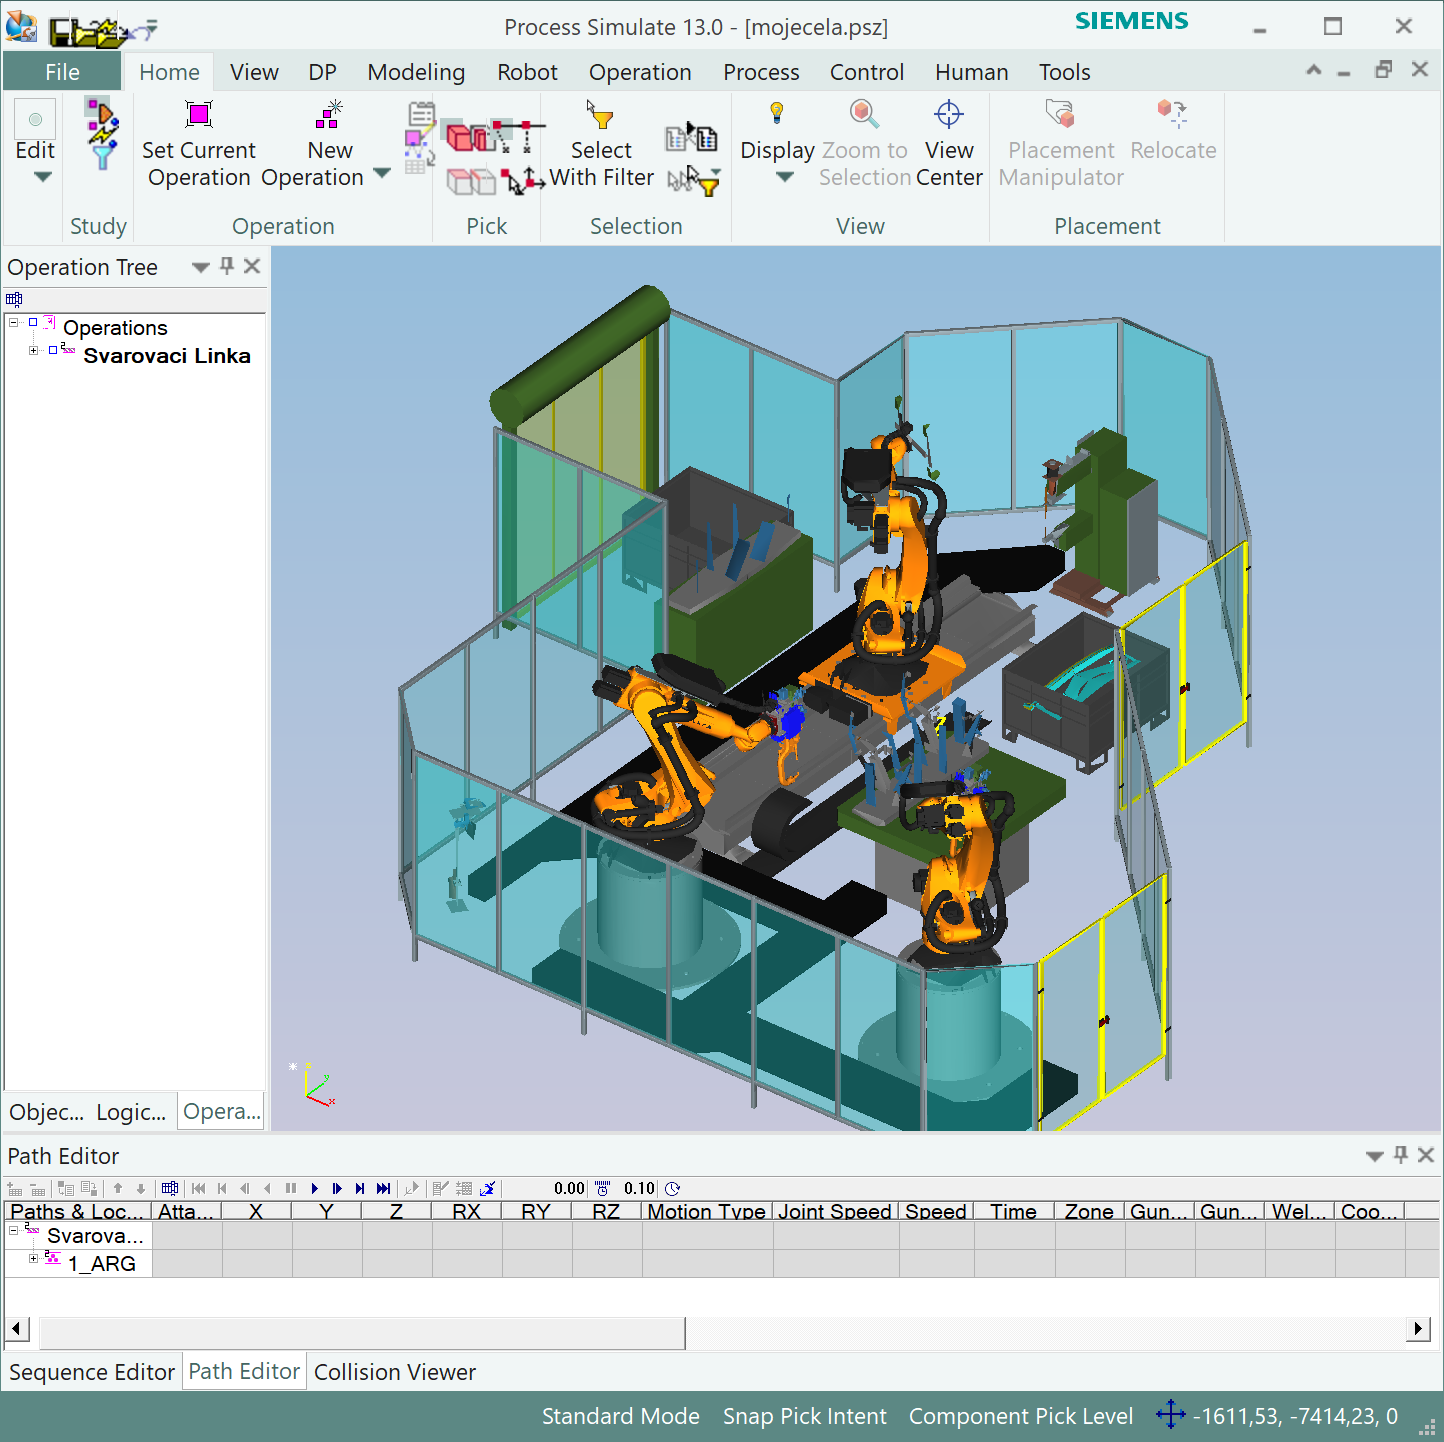
\includegraphics[width=1\textwidth]{process-simulate}
	\label{fig:ProcessSimulate}
\end{figure}

When designing an assembly line for a product the focus is on the successful creation of the product, which in itself is no mean feat. 
Then searching for the optimal layout of the robotic cell and schedule of the tasks that need to be executed for the desired result is an inhuman task. That leaves a lot of potential for computer assistance in this area. \\ 

\begin{figure}[ht]
	\caption{Industry 4.0, by Christoph Roser at AllAboutLean.com}
	\centering
	  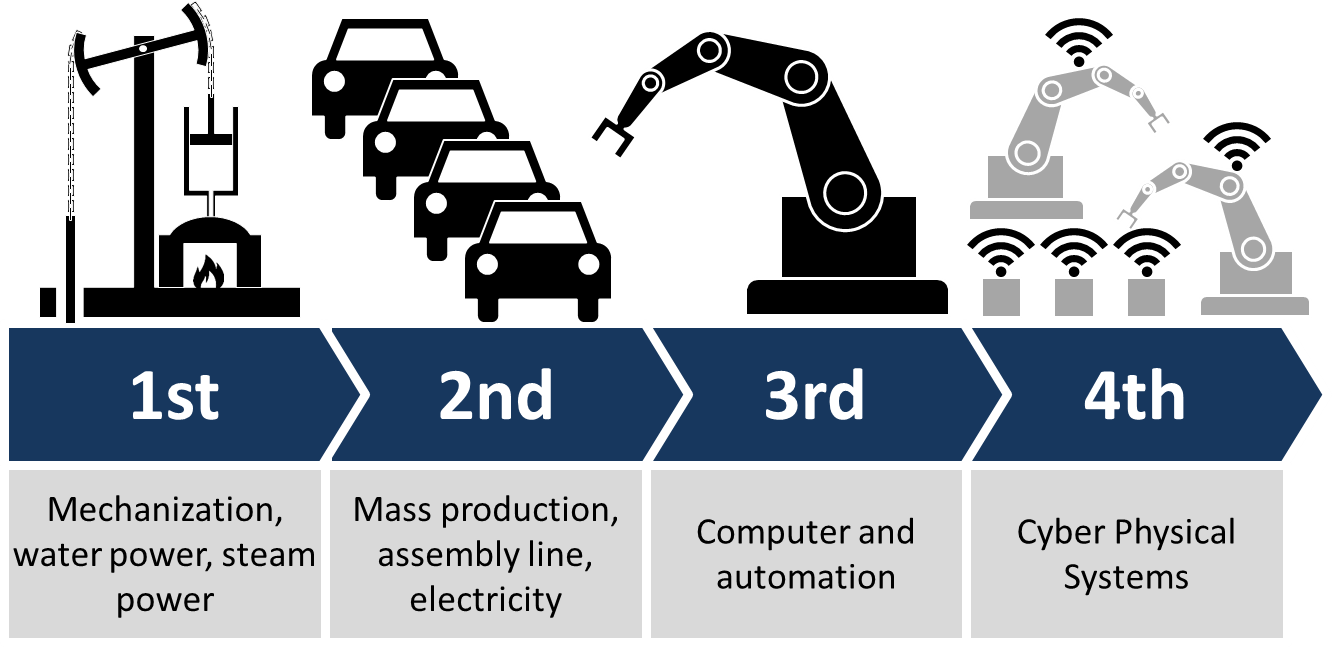
\includegraphics[width=1\textwidth]{industry-40.png}
	\label{fig:Industry40}
\end{figure}

The vision of the future, predicting the 4th industrial revolution (see figure~\ref{fig:Industry40}, was given a name "Industry 4.0". This term was popularized by the German government when they recognized the value of innovation in this field and started supporting the movement. Lasi et al. \cite{Industry40} also outline two different directions Industry 4.0 projects can take. A technological push which consists of further increasing mechanization and automation, digitization and networking, and miniaturization. Or an application pull which has mainly these areas: time to market, individualization on demand, flexibility, decentralization and resource efficiency. \\

In the context of this work the last point is the most interesting.
Resource efficiency is important for several reasons.
For example the increase of resource prices, government regulations as well as higher sensitivity to our environment. Due to these, a more intensive focus on sustainability and effectivity of the processes is required. 
The aim is an economic and ecological increase in efficiency. 

\section{Motivation}

As we touched in the previous chapter, optimization of manufacturing processes is a very interesting field with a lot of potential.

While optimizing energy usage even a small improvement could have enormous impact on the yearly savings. For example in the case of General Motors their factories drew about 9 terawatt hours in 2015 \cite{GMEnergySpending}. According to Meike et al. \cite{Meike8Percent} about 8\% of the energy used in the factories is consumed by industrial robots. Assuming consumer pricing of 10 cents per kWh even with 1 percent improvements in energy efficiency this roughly equates to \$~720000 in potential savings. In addition to that the manufacturing business is also affected by government regulations such as the plan of the European Union for energy savings \cite{EUElectricity}. \\

Another factor often optimized, which is more relevant to this work, is cycle time. Shortening the production cycles also reduces resource usage, focusing on the passive resource usage per unit (lighting, heating, employees etc.) rather than the active resource consumption (robot movement, welding etc.). \\

\section{Related Work}

Theoretical optimization of processes in robotic cells, due to the remarkable improvements, is not revolutionary. Due to its raw scale, the optimization is most pronounced in the automotive industry. However, the concepts translate to all different kinds of industries. All sorts of factors can be optimized. For example, as shown by R. G. Fenton et al. \cite{OptimizationCycleTimeFenton}, the location of the robots in a robotic cell can have a profound effect on the cycle time. It is possible to obtain the optimal position using a numerical optimization routine and a kinematic computer graphics simulation program. \\

Interfacing with a program capable of kinematic simulation, like Process Simulate, can add a lot of value to the optimization process. Certain subtleties of the domain are more straightforward to simulate rather than to capture them in a mathematical model which could make it difficult to mine it from the application and to compute the optimal solution. \\

Another approach to optimizing the cycle time of robotic cells was shown by Jiafan Zhang et al. \cite{OptimizationCycleTimeZhang}. In their research, the focus was laid mainly on scheduling movement of robots with single or dual grippers. The throughput of most dual-gripper robots can be improved using the method their team has presented in this article. 

Moreover, recently Edvin Åblad et al. \cite{CollisionAvoidanceAblad} took a look at the practical challenges of real assembly line designs. 
Rather than focusing on certain parts of the robot movement, this group chose to tackle a different factor influencing the cycle time. Collisions, which are another problem relevant to this thesis, are avoided by introducing synchronization schemes among the robots. 
These synchronization locks are preventing shared volumes of the workspaces to be simultaneously entered, which is a safe way of avoiding issues. On the other hand, it also has a negative impact on the cycle time. Edvin and the team show a new approach to maximizing throughput while eliminating all synchronizations among robots. \\

With the collaboration with one of the top players in the automotive industry, Davis Meike et al. \cite{Meike8Percent} investigates potential energy savings on robotic assembly lines for the automotive industry. Davis and the team present two practical methods for reducing the overall energy consumption. The methods entail the implementation of energy-optimal trajectories obtained utilizing time scaling, concerning the robots' motion from the last process point to the home positions and reduction of energy consumption by releasing the actuator brakes earlier when the robots are kept stationary. Notable are also the results which were simulated based on input from a real manufacturing plant. In the future, it's likely that some manufacturers might choose even to sacrifice cycle time to reach higher energy efficiency of the factory. \\

Building on top of the work of Meike et al., this study by L. Bukata et al. \cite{EnergyOptimisationBukata} focuses more narrowly on the energy optimization of industrial robotic cells. They have devised a mathematical model, which takes into account various robot speeds, positions, power-saving modes, and alternative orders of operations. Furthermore, a mixed-integer linear programming formulation is included, ready to be used. Due to speed concerns, they also created a hybrid heuristic capable of utilizing multi-core processors. Experiments show that theoretically, the energy consumption can be reduced by as much as 20\% merely by optimizing the robot speeds and applying power-saving modes. \\

Due to the diversity of the methods and objectives, which all lead to an improved manufacturing process, I recognized that the plugin must be modular and flexible enough so that the user can select different optimization cores focusing on a particular objective. \\

Anne-Laure Coiffier \cite{AnneBacktracking} wrote a thesis, which also focuses on the Tecnomatix suite of tools. The goal of her work was to find an optimal schedule for a given setup of a robotic cell and a set of operations. In comparison to my work, her approach was to assign tasks to robots, whereas I consider a fixed assignment and manipulate the speed of the robots. Her algorithm performs a mapping of the operations to the given resources, taking into account the material flow. The optimization was conducted by a Depth-First Search algorithm with backtracking rather than ILP, suggesting that a heuristic approach might be worth considering. \\

\section{Contribution}

The main contribution is the integration with the application so that optimization techniques can be brought from the academia to the industry, into the hands of the engineers. The plugin is developed as a foundation stone for future work. As such it is designed to be extendable and reusable. The integration mainly focuses on analyzing the designed robotic cell, setting up a generic optimization process, introducing helpers to get more information from the system and finally adjusting the robotic cell based on results of the optimization. \\

The work is divided into six chapters. The \href{ch:introduction}{opening chapter} introduces the reader to the industry and defines the goals of the work. The \href{ch:problem_statement}{second chapter} breaks down the problem at hand and establishes formal notation which is used throughout the rest of the work. \href{ch:milp_model}{After that} a MILP model is devised which can be used with a generic solver to provide an optimal solution minimizing cycle time. \href{ch:interface}{Then in chapter}~\ref{ch:interface} I introduce Process Simulate and explain in detail its inner workings. The \href{ch:integration}{chapter after that} focuses on the plugin itself from features to architecture. This chapter is especially important because the plugin is meant to be expandable and reusable for future work. \href{ch:experiments}{The Second to last chapter} is dedicated to a formal validation of the work. The MILP model is benchmarked, and the plugin itself is tested by the users. And finally a \href{ch:conclusion}{conclusion} is made with the recommendations for future work.    